
%
%\documentclass[onecolumn, a4paper,draftcls,twoside, 11pt]{IEEEtran}
\documentclass[journal]{IEEEtran}
% If IEEEtran.cls has not been installed into the LaTeX system files,
% manually specify the path to it like:
% \documentclass[12pt,journal,compsoc]{../sty/IEEEtran}

\usepackage{times}
\usepackage{nomencl}
\usepackage{epsfig}
\usepackage{graphicx}
\usepackage[fleqn]{amsmath}
\usepackage{amssymb}
\usepackage{subfigure}
\usepackage{booktabs}
\usepackage{url}
\usepackage{multirow}
\usepackage[linesnumbered,ruled]{algorithm2e}

 \usepackage{color}

 \newtheorem{theorem}{Theorem}[section]
\newtheorem{lemma}[theorem]{Lemma}
\newtheorem{assump}[theorem]{Assumption}
\newtheorem{problem}[theorem]{Problem}
\newtheorem{definition}[theorem]{Definition}
\hyphenation{op-tical net-works semi-conduc-tor}
\makeglossary

\begin{document}

\title{A Max-margin Recurrent Deep Neural Network to Detect Cell Phone Usage During Vehicle Driving
\thanks{ The authors are all with the Automation Department, Tsinghua University, 100084, Beijing, China. e-mail:yuedeng.thu@gmail.com.}
\thanks{
}}

\author{Zhiquan Ren, Yue Deng, Jibo He,
        and Qionghai Dai,~\IEEEmembership{Senior Member,~IEEE}}% <-this % stops a space



\markboth{DRAFT for IEEE TITS}%
{ }

\maketitle


\begin{abstract}
Despite legislative and social campaigns to reduce cell phone usage (CU) while driving, drivers continue to typing behind the wheel. In this work, we  introduced a machine learning system to detect such harmful behaviors with the recent developments of deep learning.  \textcolor{red}{Replace this sentence with a brief introduction about the simulator system: This study used a classic Lane Change Task and a smartphone detection application to study the mutual influences of driving and cell phone usage. } In the machine learning part, a max-margin recurrent deep neural network (MM-RDNN) was proposed to detect the CU from the time-course data of the vehicle sensors. The results demonstrated that our MM-RDNN is much more effective to detect the CU behaviors than  shallow and  other deep learning model. The finding of mutual interferences of driving and CU provides new knowledge for social campaigns, which intend to persuade drivers not to drive while CU, and importantly provides a scientific foundation to develop a smartphone-based technology to reduce the risky behavior of driving while CU.
\end{abstract}

\begin{IEEEkeywords}
Cell phone usage, distrsction when driving learning,  deep learning, neural network for transportation.
\end{IEEEkeywords}

\IEEEpeerreviewmaketitle
\section*{Nomenclature}
\addcontentsline{toc}{section}{Nomenclature}
\begin{IEEEdescription}[\IEEEusemathlabelsep\IEEEsetlabelwidth{$V_1,V_2,V_3$}]
\item[AE]  Auto Encoder.
\item[BPTT] Back Propagation Through Time.
\item[CU] Cell-phone Usage.
\item [DL] Deep Learning.
\item[DNN] Deep Neural Network.
\item[RDNN] Recurrent Deep Neural Network.
\item[MM-RDNN] Max-margin RDNN.
\item[NN] Neural Network.
\end{IEEEdescription}


\section{Introduction}
Cell phone usage (CU) while driving has become a disturbingly popular and dangerous behavior. The National Safety Council  estimated that 281,000 to 786,000 crashes in 2012 involved CU. A survey by the American Automobile Association reported that 14.1\% of all drivers and 48.5\% of young drivers age 18 to 24 admitted that they use smart phones while driving.  Concurrent CU impairs driving in various ways. For example, CU while driving increases hazard response time , increases lane deviations and lane excursions, increases mental demand, increases gaze-off-road durations, causes more collisions, and raises the risks of traffic accident as many as 8 to 23 times.



 
The high risk and prevalence of CU while driving has attracted the attention of legislators, automakers, and safety researchers. How could we reduce the risks of CU while driving? Researchers and practitioners have explored many approaches to mitigate the risks of CU while driving, including illegalization, social campaigns, and technology solutions. Legislation efforts have sought to discourage the behavior by making it illegal. Social campaigns have sought to educate drivers about the risks of CU while driving. Information technology companies, cell phone manufacturers and carriers have developed technologies to mitigate the risks of CU while driving. AT\&T and T-Mobile have developed smartphone applications to discourage CU while driving, such as Drive Mode and DriveSmart.  


Despite these legislative, social and technological efforts and the associated risks, drivers continue to CU while driving.  It is natural to ask: if there a more intellegent manner to detect such harmful distraction?   In addressing such a challenge, in this paper, we implement a driving simulator system to carefully study the interactions of driving and CU.
\textcolor{red} {ADD a paragraph summarizing the simulator and the data acquisition system}.


Can we learn the CU from these  sensory data from vehicle? It is another confronting challenge that requires intelligent solutions. When analyzing the specific data structure from the transportation system,  the major difficulties mainly stem from the following three aspects: 1) noise, 2) memory effect \cite{kim2003autonomous} and 3) discriminant structure . First, the data themselves were acquired from the real driving condition that may potentially contain unpredictable noises from the real-world. It hence requires the machine learning system to correctly detect the useful information from really noisy measurement. Secondly, the sensory data are in the time-course structure which are not independent overtime. Practically, the lerning system should also take such memory effects of driving vehicle statues into consideration. Thirdly, the detection task is cast into a binary classification framework and thus requires the learned feature exhibit obvious discriminative structure to facilitate the subsequent data understanding. 

In addressing the aforementioned three issues,  we propose a max-margin recurrent deep neural network (MM-RDNN) to identify the CU behaviors from vehicle data. The bulk of our MM-RDNN is mainly implemented into a recurrent deep neural network structure. The deep learning part automatically   extract informative features from the noisy input data. The recurrent structure further combine the historic memory into consideration. Finally, we have proposed a max-margin penalization term at the last hidden layer of the system to encourage the discriminant structure of the learned features. To the best of our knowledge, this is the first deep learning system that combines the max-margin objective into a recurrent  neural network structure for enhanced discriminative learning.  The MM-RDNN is trained by the back-propagation through time (BPTT) algorithm that is particularly effective in practice.

 
 



\section{Related Works}

The lack of understating about CU performance is possibly because CU performance is less vital compared to driving performance or because it is hard to collect and evaluate CU performance before the invention of smartphone. The changes of driving, and also CU performance may have important theoretical implication and practical application.  When drivers write text messages while driving, do they divide their attention or switch attention between driving and CU task? The attention allocation strategy can have a great influence on dual task performance. The research group at University of Utah hypothesized that ?CU messaging appears to be most consistent with a switching model of attention?. That is, drivers either drive or text. In contrast, they hypothesized that cell phone conversation appears to be a sharing model of attention. Whether CU while driving is better explained by an attention-switching model or an attention-sharing model needs more evidence. Analyses of both driving and CU performance may provide more information about the underlying attentional strategy for CU while driving. Practically, if we have a better understanding of CU performance, we may be able to develop a smartphone application that can detect and stop instances of CU while driving. Several researchers are beginning to explore smartphone applications that can monitor impaired driving condition, and showed promising opportunities to use smartphone technology to improve driving safety.


As many as 91\% of college students reported having sent text messages while driving, even though they agreed that CU while driving was dangerous and should be illegal. Evidence for the effectiveness of legal prohibitions of CU while driving is mixed.  McCartt et al. (2010) found that bans in the District of Columbia (D.C.), New York, and Connecticut reduced handheld phone use over time, however this could be partially due to an increase in the use of hands-free devices. Evidence indicates that state anti-CU laws have little effect on the likelihood of a teenager to text while driving, with 39 percent of teens reporting CU in states where it is illegal compared to 44 percent of teens in states that have no restrictions. Despite legislative efforts to curb CU while driving, many drivers will continue to do so.

According to the theories of dual-task performance, when two tasks are carried out concurrently, the performances of one or both tasks may be impaired, causing a dual-task performance decrement. Although both tasks may be impaired, most driving studies focus on driving performance, while CU performance is mostly ignored or less emphasized. Smartphones allow researchers to collect detailed data on secondary task performance. In this study, we utilize the capability of smartphones to capture CU performance and describe the mutual interferences of CU and driving. This assess intends to describe the two facets of CU while driving, inform the theory of dual-task performance, and provide evidence for social campaigns and technology innovations to reduce the risks of CU while driving.

Driver distraction is one of the major factors, which contribute to vehicle crashes and casualties (J. He et al., 2014; Jibo He, Choi, McCarley, Chaparro,  Wang, 2015; Strayer, Drews, Johnston, 2003). Various approaches have been made to detect driver distraction(Liang, Lee,  Reyes, 2007; Liang, Reyes,  Lee, 2007), drunk driving(Lee et al., 2010), and drowsy driving(Jibo He, Choi, Wu,  Yang, 2015; You et al., 2013). Existing work has explored using vehicle dynamics(Jin et al., 2012; Lee et al., 2010; Sayed  Eskandarian, 2001), head movements(J. He et al., 2013; Murphy-Chutorian, Doshi,  Trivedi, 2007), eye movements(Liang, Reyes, et al., 2007), and wearable devices? proximity sensor(Jibo He, Choi, Wu, et al., 2015), and infrared imaging(Koukiou  Anastassopoulos, 2012) to monitor driver impairment. Various types of machine learning approaches(Tango  Botta, 2013) have been explored to identify impaired drivers from the multidimensional input variables, such as Bayesian Network(Liang  Lee, 2014; Liang, Lee, et al., 2007), Support Vector Machine(Liang, Reyes, et al., 2007), Decision Trees(Lee et al., 2010), Neural Network(Sayed  Eskandarian, 2001; Wollmer et al., 2011), Random Forest(McDonald, Lee, Schwarz, Brown, 2013; Ragab, Craye, Kamel,  Karray, 2014). For the types of driver distractions, researchers have attempted to detect cognitive distractions (Jin et al., 2012; Liang, Reyes, et al., 2007) and visual distractions, however, the investigations of the distracting effect of texting while driving and the algorithms to detect texting while driving are seldom studied. In the current paper, we will utilize the latest Deep Learning algorithms in the field of machine learning to detect texting while driving, which is a relatively under-investigated but more destructive risky driving behavior(Caird, Johnston, Willness, Asbridge,  Steel, 2014; Drews, Yazdani, Godfrey, Cooper, Strayer, 2009; J. He et al., 2014).

\textcolor{red}{Revise the previous three paragraphs by adding the citations.}

\section{Driver Simulation System}

\textcolor{red}{Introduce driving system, and data collection system. Please add more figures as you can to illustrate the system and experiment}
\section{A Max-margin Deep Recurrent Neural Network}
\subsection{Vehicle Data Preprocessing }
We define the mathematical notations for the problem. First, we have obtained $S$ replicates of time-course data $F$ from different participants in the driving model.  For the  $s^{th}, s \in\{1...S\},$   time-course data $F^{s}=[f^s_1....f^s_T]  \in \mathbb{R}^{m\times T}$,  each time point $f^s_t$ records the sensory information from $m$ sensors describing the status of the car. Then, since the data has been synchronize with the driving simulator, it is easy to obtain the label for each distinct time point $t$ to tell whether the participant was using the cell phone $(l^s_t=1)$ or not $(l^s_t=0)$.   

In the implementation, we prefer to perform the classification on a set of time points rather than the single time point due to the following two reasons. First, the sensory data is obtained from practical driving condition which could be quite noisy. The experiments on the single point may be greatly affected by the
 noises in the measured data. The set-level classification took the whole information of a set into consideration and this contain rich information to be identified. Second, the cell-phone usage exhibit obvious memory effects. The cell phone usage in the $t^{th}$ time point may imply the same condition in the $(t-1)^{th}$ and $(t+1)^{th}$ points. Accordingly, we explicitly take the time-course information into consideration and try to detect the CU based on a set of time points. 

For the ease of the subsequent machine learning steps, we divided $F^{s}$ as $\frac{T}{w}$  non-overlapping sets with the same windows size $w$.  We consider the $i^{th}$ sequential feature set acquired from the $s^{th}$ replicate as
 \begin{equation}
 d^{s}_i=[f_{(i-1)*w+1},...,f_{i*w}] \in \mathbb{R}^{m\times w}.
 \label{eqs:d}
 \end{equation}
 To note, the CU label $l^{s}_i$ is assigned at the time-point resolution while not on the set level.  To assign the label to each divided set, we adopted the majority voting strategy to assign  $L^{s}_i=1$ (for the $i^{th}$ set) if most time-point level labels $l^{s}$ in this set is 1; and $L^{s}_i=0$ otherwise. 

\subsection{Recurrent Deep Neural Network}
The acquired vehicle data are noisy and exhibit sequential structure. To fully understand the inherent information behind the data, a max-margin recurrent deep neural network structure was established in Fig.\ref{fig:overview}.  The bulk of this deep learning infrastructure is composed of three parts: deep feature transformation (black),  recurrent (red), task driven learning (yellow) and max margin discriminant enhancement (purple) parts. We will illustrate the implementations of theses four parts sequentially.  
\begin{figure}[!htp]
  \centering
    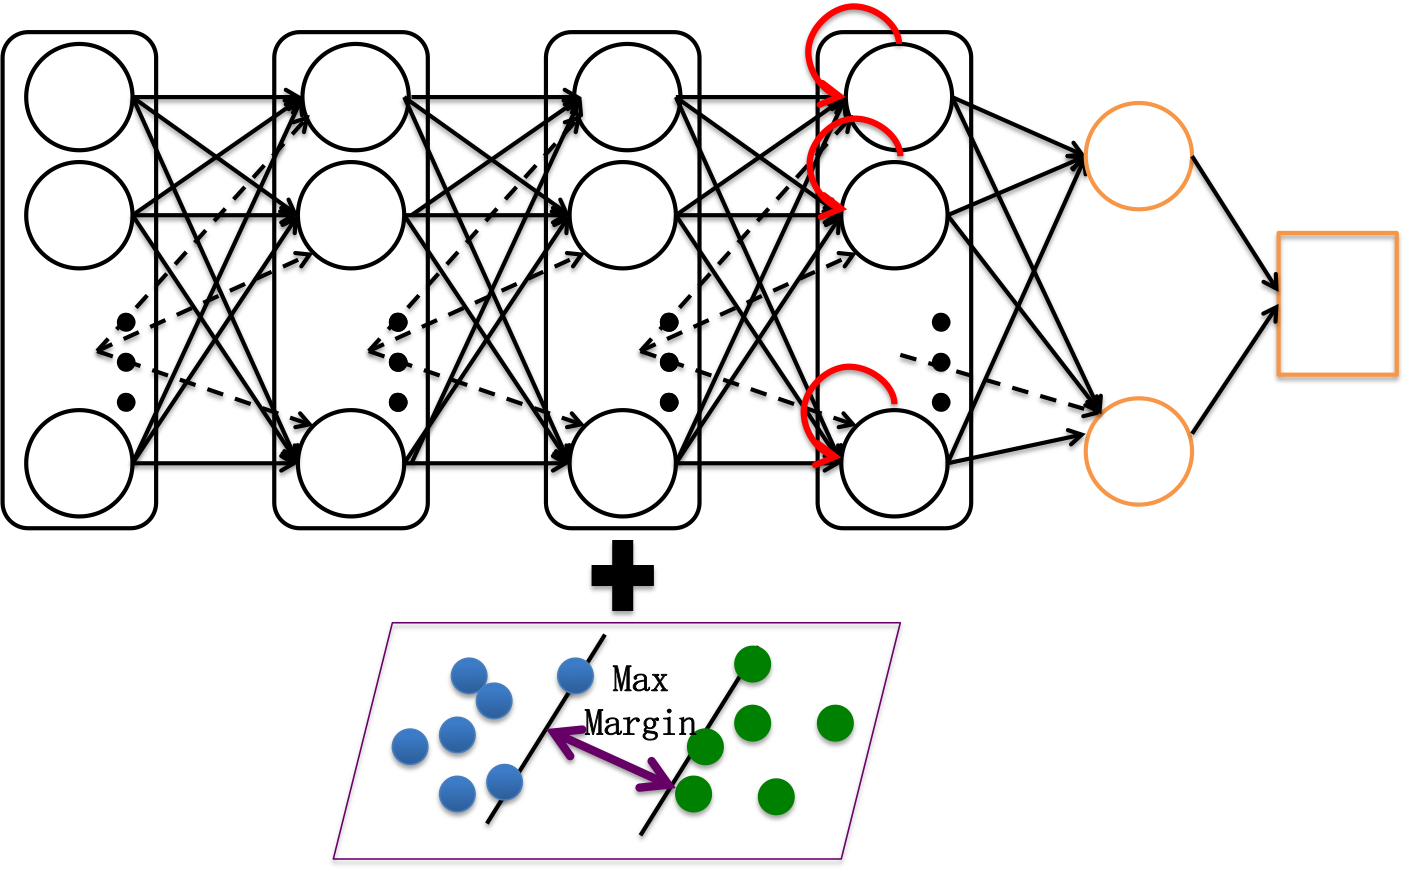
\includegraphics[width=0.95\linewidth]{overview.png}
  \caption{The configuration of the max-margin recurrent deep neural network. }
\label{fig:overview}
\end{figure}

\textbf{Deep Transformation:} The deep feature transformation part is composed of $k$ fully densely-connected hidden layers. The first layer of this part is the input layer coming from the high-dimensional vehicle data $d^{s}_i$ in (\ref{eqs:d}). For each hidden node on these deep layers, it linearly combines  all the nodes' output from its pervious layer and then follow a rectified linear unit (ReLU) to restrict  the energy of the linear transformation. The implementation of this  deep transformation part is the same as existing benchmark deep nerual network settings in the field \cite{AE}, which have been proved to be effective learning paradigm to remove the noise from the input data.

\textbf{Recurrent Layer:} The recurrent layer is almost the same as the deep transformation layer except for a number of feedback links (red links in Fig.\ref{fig:overview}).  For the $k^{th}$ hidden node on the recurrent layer, its output is defined as:
\begin{equation}
h^{(l)}_k[t]=\mathcal{H}\{\sum_i w_{ik} h^{(l-1)}_i[t]+\theta_k h^{(l)}_k[t-1] +b\},
\label{eqs:recurrent}
\end{equation}
where $h^{(l)}_k[t]$ is the output of the hidden node at time $t$, $w_ik$ defines the connecting weight from the $i^{th}$ node's ($l-1$ layer) output to the $k^{th}$ node on the recurrent layer ($l$ layer), $\theta_k$ is the weight of the memory effect (reccurrent link ) and b is the bias term. $\mathcal{H}\{\cdot\}$ is the ReLU nonlinear transformation.

\textbf{Task-driven learning:} The task driven part accumulated across the output of $w$ sequential input and then form a probability in each category. In detail, this part firstly linear combine the outputs of the recurrent layer as:
\begin{equation}
A_L=\sum_{t=1}^w O[t]=\sum_{t=1}^w\sum_i (W^{L}_i h^{(l)}_i[t]+b),
\end{equation}
where L is the binary label: $L=1$ (cell phone usage) and $L=0$ (no cell phone usage). Then, the final probabilistic output of the deep neural network can be defined as:
\begin{equation}
P(L)=\frac{exp(A_{L})}{\sum_{l=0}^{1}exp(A_l)}.
\end{equation}


\subsection{A max-margin Extension}
The discussions in the last subsection have stated the general framework of deep recurrent neural network. By exploiting the RDNN, two issues of data noise and memory effect can be fully addressed. In this part, we further improve the performances of RDNN by incorporating the max-margin penalty into  the learning system to further enhance the discriminant of the learned features.



\textbf{Max-margin part:} The max-margin penalty was added at the last recurrent layer of the RDNN. It encourage the learned feature to stay as far as possible if their labels are not the same. In machine learning, this pursuit has been well formulated via the max-margin loss.  To illustrate the penalty, we define $H^{(l)}_s[t]$ as the output vector of the hidden representation at the output layer for the $s^{th}$ participant, and $L^s$ is the Cell phone usage label of the participant.  The, we define the loss as:


\begin{equation}
\mathcal{C}_s=
\begin{cases}
\sum_t\|H^{(l)}_s[t]-H^{(l)}_j[t]\|_2^2,  L_s=L_j\\
\sum_t \max(0,d-\|H^{(l)}_s[t]-H^{(l)}_j[t]\|_2^2)  L_s \neq L_j
\end{cases}
\end{equation}

This term penalize the distances of hidden representations in different classes. When two samples' label are the same, their distances are encouraged to be as small as possible. On the contrary, when they are from different classes, their coherent  distance is penalize to be far away from each other with a margin $d$. In max-margin learning systems, $d$ is a  constant as is always fixed  as one.

Till now, we can define the whole learning objective of the MM-RDNN as
\begin{equation}
\mathcal{Y}(d^s)= \sum_{s=1}^{S} \{ \ln(\sum_k \delta(k-L)P(l)) +C_s\}
\end{equation}
where L denotes the ground truth label


Backward pass: We use the back-propagation through time (BPTT) algorithm \cite{BPTT} to obtain the derivatives of the objective function with respect to all the weights, and minimize the objective function by stochastic gradient de- scent.
\section{Experiments}
\subsection{Experimental Setup}
\textcolor{red}{Show some data from the our system}


  \bibliographystyle{ieeetran}
\bibliography{egbib}



\end{document}
